\subsection{Tutorial}
Il tutorial di seguito è possibile anche trovarlo al link: \href{https://github.com/Wabri/ATTSW_Exam/tree/issue-31/gradle.example/fourth}{\texttt{github.com/Wabri/ATTSW\_Exam/tree/issue-31/gradle.example/fourth}}.
\begin{enumerate}
    \item Creare una repository su github e clonarla localmente:
    \begin{figure}[H]
    \centering
    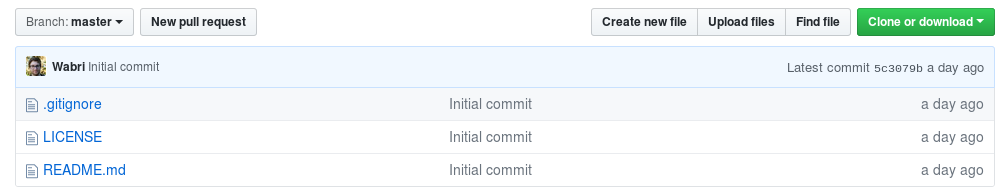
\includegraphics[width=1\linewidth]{4IntegrationWithOtherTool/tutorial/githubRepo.png}
    \end{figure}
    \item Nella repository locale creare una cartella chiamata tutorial:
    \begin{figure}[H]
    \centering
    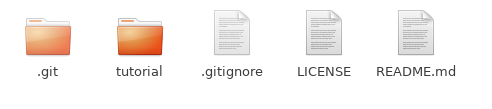
\includegraphics[width=0.7\linewidth]{4IntegrationWithOtherTool/tutorial/localGithubRepo.png}
    \end{figure}
    \item Spostarsi nella cartella appena creata e eseguire la build Gradle \texttt{init} per una applicazione java:
    \begin{verbatim}
        $ gradle init --type java-application
    \end{verbatim}
    \begin{figure}[H]
    \centering
    
\includegraphics[width=0.8\linewidth]{4IntegrationWithOtherTool/tutorial/gradleInit.png}
    \end{figure}
    \item Modificare il build.gradle sostituendolo con questa versione:
    \begin{lstlisting}[frame=single]
plugins {
    id 'java'
    id 'application'
    id 'eclipse'
}

mainClassName = 'App'

repositories {
    mavenCentral()
}

dependencies {
    testImplementation 'junit:junit:4.12'
}

task  wrapper(type: Wrapper) {
    gradleVersion = '4.6'
    distributionType = Wrapper.DistributionType.ALL
}
    \end{lstlisting}
    Con questo setting del file build abbiamo impostato sia il plugin di eclipse sia la distribuzione del wrapper da usare.
    \item Aggiornare quindi il wrapper con la build relativa:
    \begin{verbatim}
        $ ./gradlew wrapper
    \end{verbatim}
    \item Creare i meta dati di eclipse con la build omonima definita dal plugin stesso:
    \begin{verbatim}
        $ ./gradlew eclipse
    \end{verbatim}
    \item Possiamo ora importare la repository su Eclipse:
    \begin{figure}[H]
    \centering
    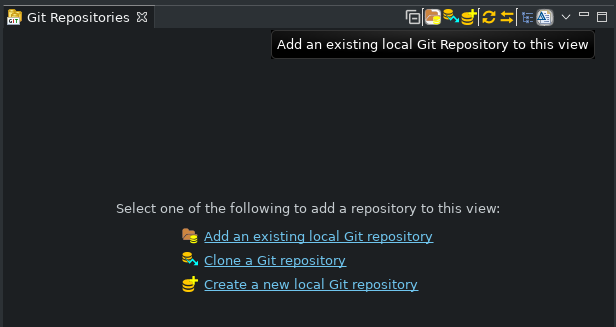
\includegraphics[width=0.8\linewidth]{4IntegrationWithOtherTool/tutorial/addExistingLocalGitRepository.png}
    \end{figure}
    \item Importare poi il progetto creato sulla repository:
    \begin{figure}[H]
    \centering
    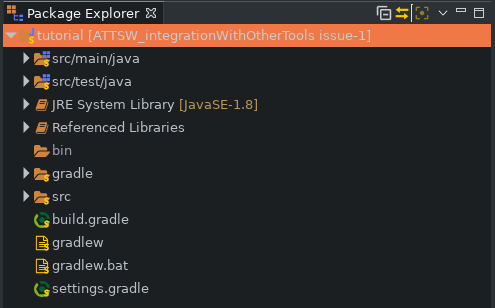
\includegraphics[width=0.8\linewidth]{4IntegrationWithOtherTool/tutorial/localRepositoryEclipse.png}
    \end{figure}
    \item Effettuare il login su \textbf{\href{https://travis-ci.org}{travis-ci.org}} e aggiungere la repository Github creata:
    \begin{figure}[H]
        \centering
        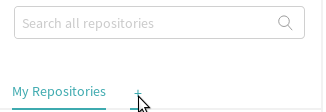
\includegraphics{4IntegrationWithOtherTool/tutorial/newTravis.png}
    \end{figure}
    Attivare la repository:
    \begin{figure}[H]
        \centering
        
\includegraphics{4IntegrationWithOtherTool/tutorial/spuntaTravis.png}
    \end{figure}
    Andare nelle impostazioni della repository:
    \begin{figure}[H]
    \centering
    
\includegraphics{4IntegrationWithOtherTool/tutorial/settingsTravis.png}
    \end{figure}
    E indicare al server di eseguire la build solo nel caso in cui ci sia il travis.yml:
    \begin{figure}[H]
    \centering
    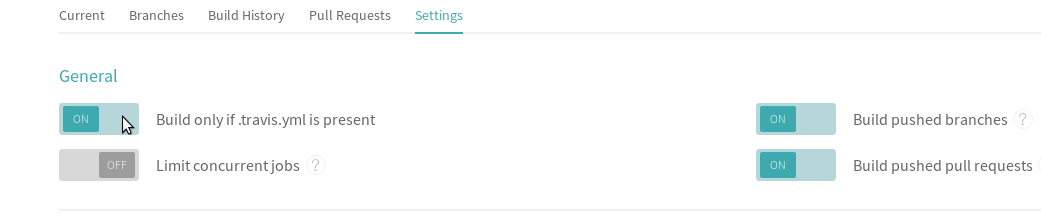
\includegraphics[width=0.7\linewidth]{4IntegrationWithOtherTool/tutorial/buildOnlyTravis.png}
    \end{figure}
    \item Creaiamo il file \texttt{travis.yml} nel quale andremo a indicare la build da eseguire, impostiamo quindi il file in questo modo:
    \begin{minted}[gobble=4, frame=single, linenos]{yaml}
    language: java

    jdk:
        - oraclejdk8
        - oraclejdk9

    # cache settings
    before_cache:
        - rm -f  $HOME/.gradle/caches/modules-2/modules-2.lock
        - rm -fr $HOME/.gradle/caches/*/plugin-resolution/
    cache:
        directories:
            - $HOME/.gradle/caches/
            - $HOME/.gradle/wrapper/

    script:
        - ./tutorial/gradlew --no-daemon -b tutorial/build.gradle test
  \end{minted}
  Salvando ed aggiornando potremmo vedere che Travis inizierà ad eseguire la build specificata nel file appena creato. Il risultato dovrebbe essere qualcosa di simile:
  \begin{figure}[H]
    \centering
    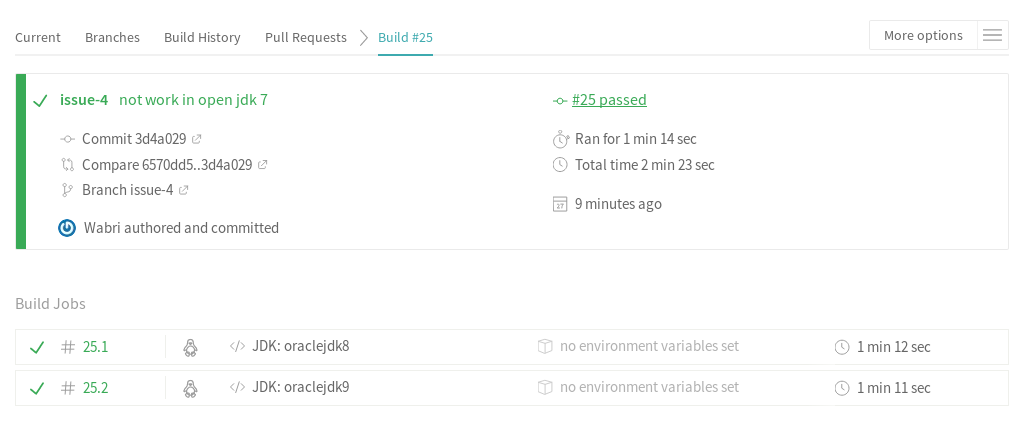
\includegraphics[width=0.9\linewidth]{4IntegrationWithOtherTool/tutorial/verifyBuild.png}
  \end{figure}
  \item Possiamo importare il tag dello stato della build nel README della repository per ottenere:
  \begin{figure}[H]
    \centering
    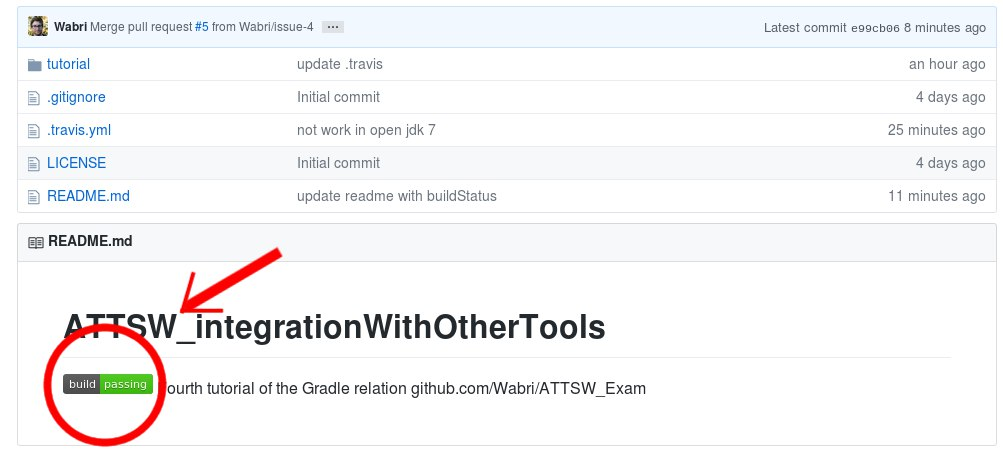
\includegraphics[width=0.8\linewidth]{4IntegrationWithOtherTool/tutorial/tagBuildPass.jpg}
  \end{figure}
  Nella build di travis accanto al nome della repository c'è questo tag:
  \begin{figure}[H]
    \centering
    
\includegraphics[width=0.2\linewidth]{4IntegrationWithOtherTool/tutorial/buildPassTag.png}
  \end{figure}
  Cliccandoci si apre una finestra in cui potrete scegliere il branch e la modalità di import, nel nostro caso avremo bisogno del codice markdown che corrisponderà ad una istruzione di questo tipo: 
    \begin{minted}[gobble=4, frame=single, linenos]{yaml}
     [![Build Status]
     (https://travis-ci.org/<User>/<gitRepositoryName>.svg?branch=master)]
     (https://travis-ci.org/<User>/<gitRepositoryName>))
  \end{minted}
  Copiamo e incolliamo (con le dovute modifiche) direttamente nel README.md ottenendo il risultato mostrato sopra.
  \item Prima di proseguire con un esempio pratico importiamo la dipendenza Mockito utile per i test successivi:
  \begin{lstlisting}[frame=single]
dependencies {
    testImplementation 'junit:junit:4.12'
    testImplementation 'org.mockito:mockito-core:2.18.0'
}\end{lstlisting}
    \item Nei passi successivi si consiglia di creare un nuovo branch per poter vedere meglio la funzionalità di Travis. Lo schema delle classi da creare è il seguente:
    \begin{figure}[H]
    \centering
    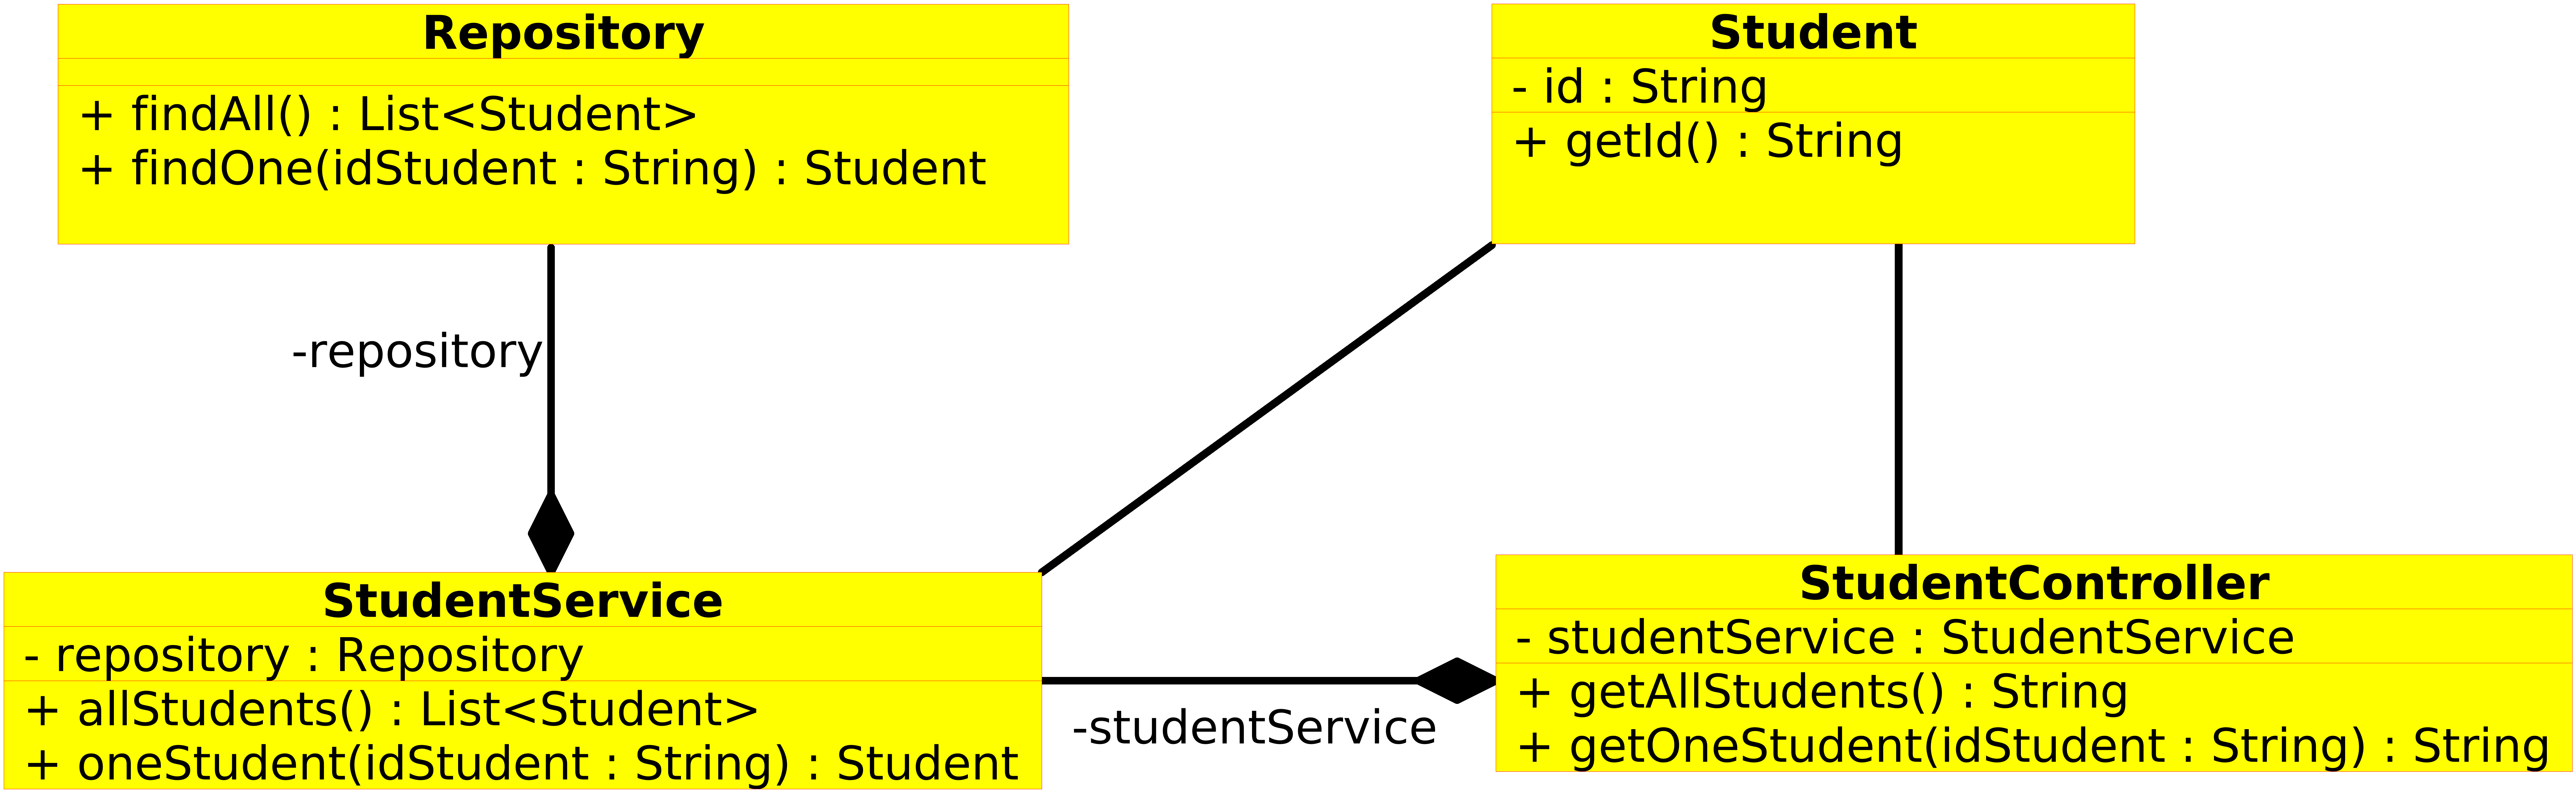
\includegraphics[width=0.8\linewidth]{4IntegrationWithOtherTool/tutorial/classDiagram.png}
  \end{figure}
  Il codice di test di StudentService è:
  \begin{lstlisting}[frame=single]
import static org.junit.Assert.*;
import static org.mockito.Mockito.*;

import java.util.ArrayList;
import java.util.List;

import org.junit.Before;
import org.junit.Test;

import attsw.exam.example.core.repository.Repository;
import attsw.exam.example.core.service.StudentService;

public class StudentServiceTest {

	StudentService studentService;
	List<Student> studentsList;
	Repository repository;

	@Before
	public void init() {
		studentsList = new ArrayList<Student>();
		repository = mock(Repository.class);
		studentService = new StudentService(repository);
		when(repository.findAll()).thenReturn(studentsList);
	}

	@Test
	public void testAllStudentsWithNoStudents() {
		verifyNumberOfStudents(0);
	}

	@Test
	public void testAllStudents() {
		studentsList.add(newStudentTest("id0"));
		studentsList.add(newStudentTest("id1"));
		verifyNumberOfStudents(2);
	}

	@Test
	public void testOneStudentWhenStudentsIsEmpty() {
		when(repository.findOne("id0")).thenReturn(null);
		assertNull(studentService.oneStudent("id0"));
		verify(repository, times(1)).findOne("id0");
	}

	@Test
	public void testOneStudent() {
		when(repository.findOne("id0")).thenReturn(newStudentTest("id0"));
		Student oneStudent = studentService.oneStudent("id0");
		assertNotNull(oneStudent);
		assertEquals("id0", oneStudent.getId());
		verify(repository,times(1)).findOne("id0");
	}

	private Student newStudentTest(String idStudent) {
		return new Student(idStudent);
	}

	private void verifyNumberOfStudents(int expected) {
		assertEquals(expected, studentService.getAllStudents().size());
		verify(repository, times(1)).findAll();
	}

}
  \end{lstlisting}
  Il codice di test di StudentController è:
   \begin{lstlisting}[frame=single]
import static org.junit.Assert.*;
import static org.mockito.Mockito.*;

import java.util.ArrayList;
import java.util.List;
import java.util.stream.Collectors;

import org.junit.Before;
import org.junit.Test;

import attsw.exam.example.core.controller.StudentController;
import attsw.exam.example.core.service.IStudentService;

public class StudentControllerTest {

	StudentController studentController;
	private List<Student> studentsList;
	private IStudentService iStudentService;

	@Before
	public void init() {
		studentsList = new ArrayList<Student>();
		iStudentService = mock(IStudentService.class);
		when(iStudentService.getAllStudents()).thenReturn(studentsList);
		studentController = new StudentController(iStudentService);
	}

	@Test
	public void testGetAllStudentsWhenThereAreNoStudents() {
		assertGetAllStudent("");
	}

	@Test
	public void testGetAllStudents() {
		studentsList.add(newStudentTest("id0"));
		studentsList.add(newStudentTest("id1"));
		assertGetAllStudent(extractAllStudentsStringFromList(studentsList));
		verify(iStudentService, times(1)).getAllStudents();
	}

	@Test(expected = NullPointerException.class)
	public void testGetOneStudentWhenThereAreNoStudents() {
		assertNull(studentController.getOneStudent("id0"));
	}

	@Test
	public void testGetStudent() {
		Student student = new Student("id0");
		when(iStudentService.oneStudent("id0")).thenReturn(student);
		assertEquals(student.toString(), studentController.getOneStudent("id0"));
		verify(iStudentService, times(1)).oneStudent("id0");
	}

	private String extractAllStudentsStringFromList(List<Student> list) {
		return list.stream().map(student -> student.toString() + System.getProperty("line.separator"))
				.collect(Collectors.joining());
	}

	private void assertGetAllStudent(String expected) {
		assertEquals(expected, studentController.getAllStudents());
		verify(iStudentService, times(1)).getAllStudents();
	}

	private Student newStudentTest(String idStudent) {
		return new Student(idStudent);
	}

}
  \end{lstlisting}
  A partire da queste 2 classi di test è possibile ricavarsi l'implementazione del codice completo. A questo punto si ha un codice effettivo in cui Travis può eseguire la sua build precedentemente impostata.
  \item Andiamo ora a generare dei report sul codice appena scritto, per farlo aggiungiamo ai plugin di Gradle sia Jacoco che Sonarqube:
    \begin{lstlisting}[frame=single]
plugins {
    id 'java'
    id 'application'
    id 'eclipse'
  	id "org.sonarqube" version "2.6"
  	id 'jacoco'
}

mainClassName = 'App'

repositories {
    mavenCentral()
}

dependencies {
    testImplementation 'junit:junit:4.12'
    testImplementation 'org.mockito:mockito-core:2.18.0'
}

task  wrapper(type: Wrapper) {
    gradleVersion = '4.6'
    distributionType = Wrapper.DistributionType.ALL
}

sonarqube {
    properties {
        property "sonar.projectName", "Java :: tutorial :: SonarQube Scanner for Gradle"
        property "sonar.jacoco.reportPath", "${project.buildDir}/jacoco/"
    }
}
    \end{lstlisting}
    Per eseguire Sonarqube useremo un contenitore server di Docker che genererà una pagina accessibile direttamente dal browser, inoltre Sonarqube avrà bisogno di un database server che creeremo sempre con Docker. Jacoco verrà usato da Sonarqube per generare il rapporto di code coverage. Entrambi i server verranno eseguiti compilando un docker-compose, per poter compilare ed eseguire entrambi i server Docker è necessario installare sia docker che docker-compose. All'interno della cartella del progetto creiamo un file chiamato \textbf{docker-compose.yml} in cui scriveremo:
    \begin{minted}[frame=single, linenos]{yaml}
version: "2"

services:
  sonarqube:
    image: sonarqube
    ports:
      - "9000:9000"
    networks:
      - sonarnet
    environment:
      - SONARQUBE_JDBC_URL=jdbc:postgresql://db:5432/sonar
    volumes:
      - sonarqube_conf:/opt/sonarqube/conf
      - sonarqube_data:/opt/sonarqube/data
      - sonarqube_extensions:/opt/sonarqube/extensions
      - sonarqube_bundled-plugins:/opt/sonarqube/lib/bundled-plugins

  db:
    image: postgres
    networks:
      - sonarnet
    environment:
      - POSTGRES_USER=sonar
      - POSTGRES_PASSWORD=sonar
    volumes:
      - postgresql:/var/lib/postgresql
      - postgresql_data:/var/lib/postgresql/data

networks:
  sonarnet:
    driver: bridge

volumes:
  sonarqube_conf:
  sonarqube_data:
  sonarqube_extensions:
  sonarqube_bundled-plugins:
  postgresql:
  postgresql_data:
  \end{minted}
  Questo file è possibile trovarlo nella pagina Github della Docker image di Sonarqube: \href{https://github.com/SonarSource/docker-sonarqube/blob/master/recipes.md}{github.com/SonarSource/docker-sonarqube/blob/master/recipes.md}. Componiamo questo contenitore andando a eseguire il comando:
  \begin{verbatim}
      $ docker-compose up
  \end{verbatim}
  Prenderà un po' di tempo, circa 3/4 minuti in base alla connessione e alla macchina su cui si sta lavorando, avrà finito quando il terminale avrà in output:
  \begin{verbatim}
sonarqube_1  | 2018.04.10 11:49:53 INFO  app[][o.s.a.SchedulerImpl] Process[ce] is up
sonarqube_1  | 2018.04.10 11:49:53 INFO  app[][o.s.a.SchedulerImpl] SonarQube is up
  \end{verbatim}
  A questo punto facciamo ripartire il contenitore, eseguendo in un altro terminale il comando:
  \begin{verbatim}
      $ docker-compose restart sonarqube
  \end{verbatim}
  Una volta completato questo comando possiamo controllare se effettivamente il server sta funzionando visitando la pagina \textbf{\href{http://localhost:9000}{localhost:9000}}:
  \begin{figure}[H]
        \centering
        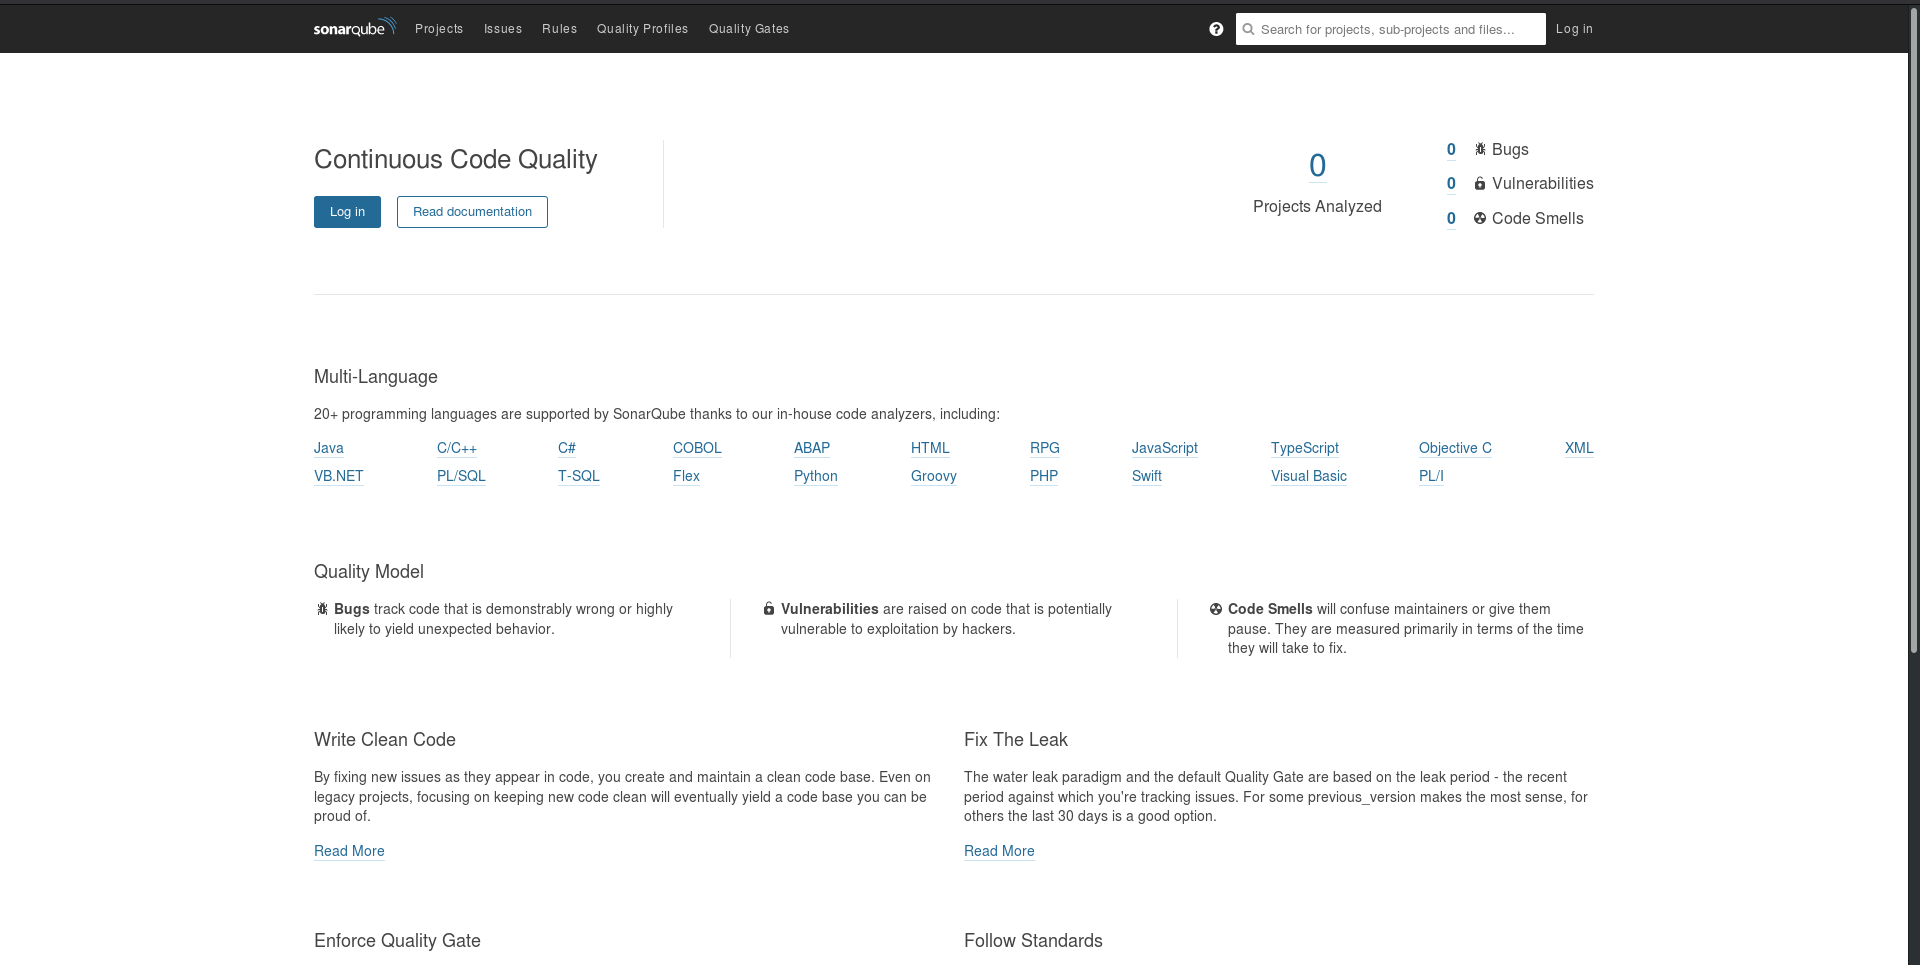
\includegraphics[width=0.8\linewidth]{4IntegrationWithOtherTool/tutorial/sonarQubeFirst.png}
    \end{figure}
    \item Dobbiamo analizzare il progetto che abbiamo creato, per farlo basterà eseguire il task sonarqube del plugin omonimo, eseguiamo quindi (da terminale o da eclipse):
    \begin{verbatim}
        $ ./gradlew sonarqube
    \end{verbatim}
    Non appena la build sarà completata Sonarqube verrà aggiornato:
    \begin{figure}[H]
        \centering
        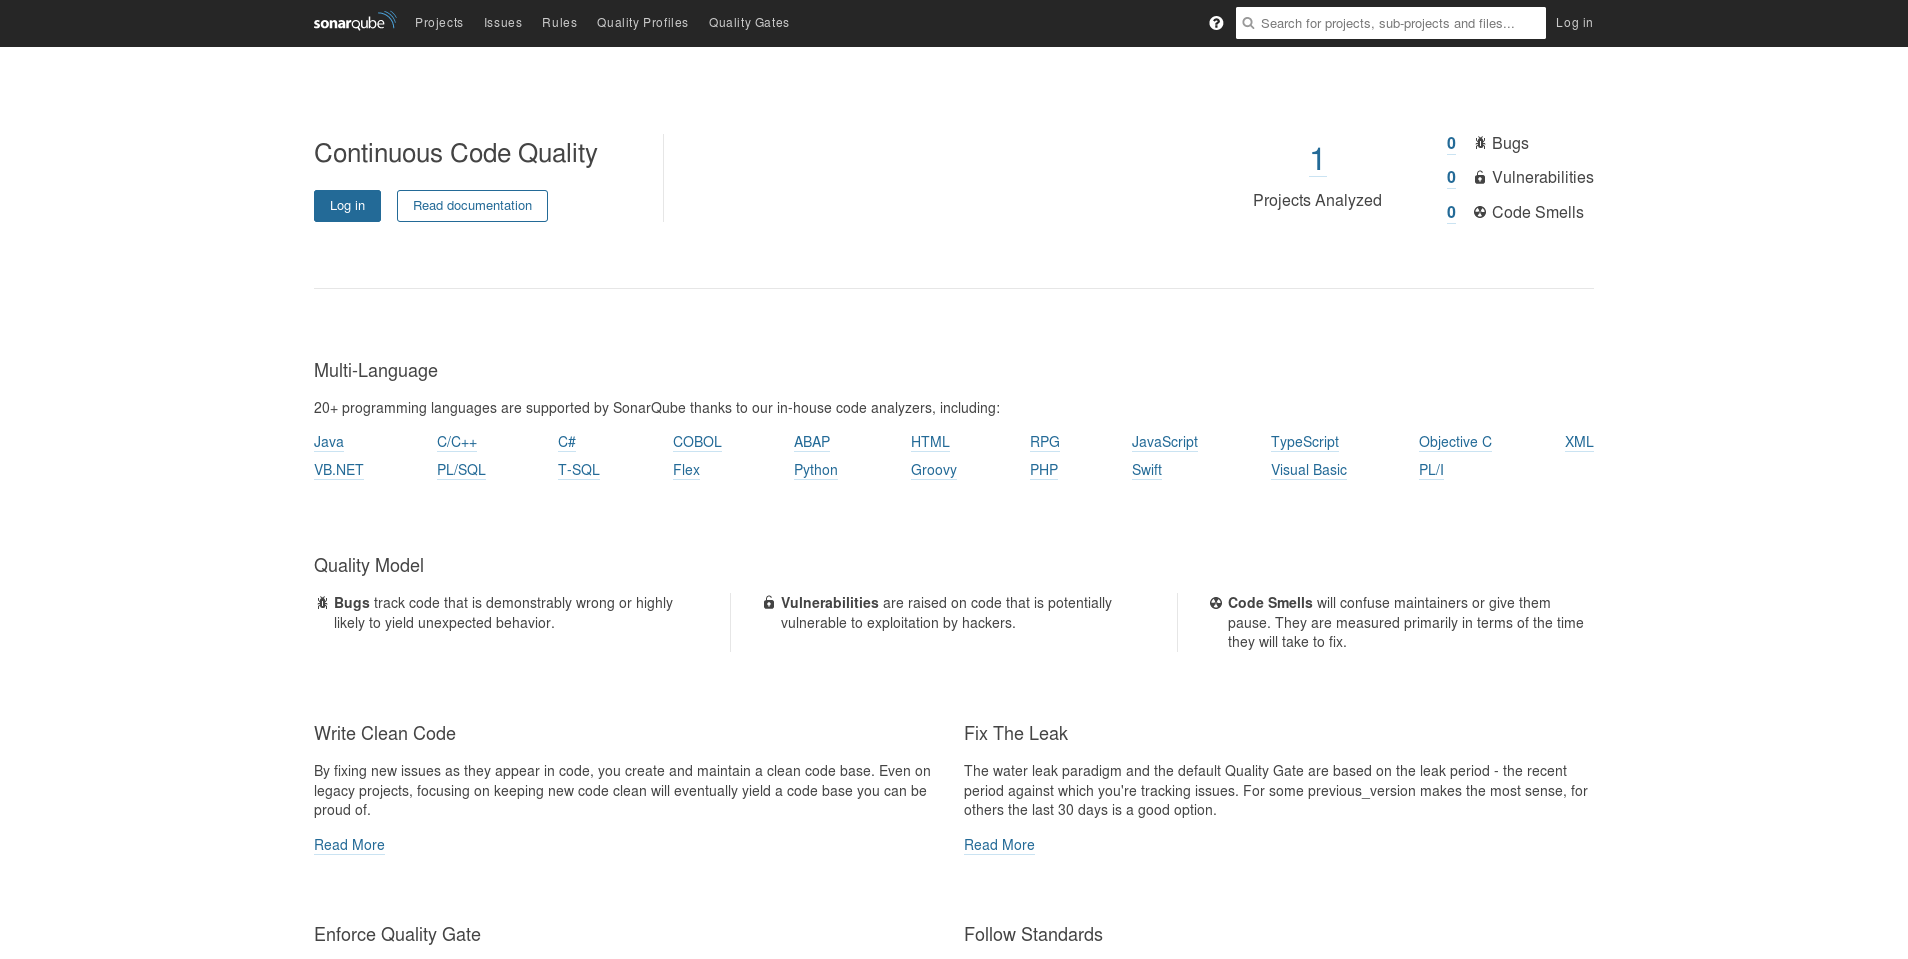
\includegraphics[width=0.8\linewidth]{4IntegrationWithOtherTool/tutorial/sonarqubeProjet.png}
    \end{figure}
    Cliccando sul numero di \texttt{Projects Analyzed} verranno mostrati i progetti analizzati e selezionando il progetto da visualizzare avremo la schermata di report del nostro progetto:
    \begin{figure}[H]
        \centering
        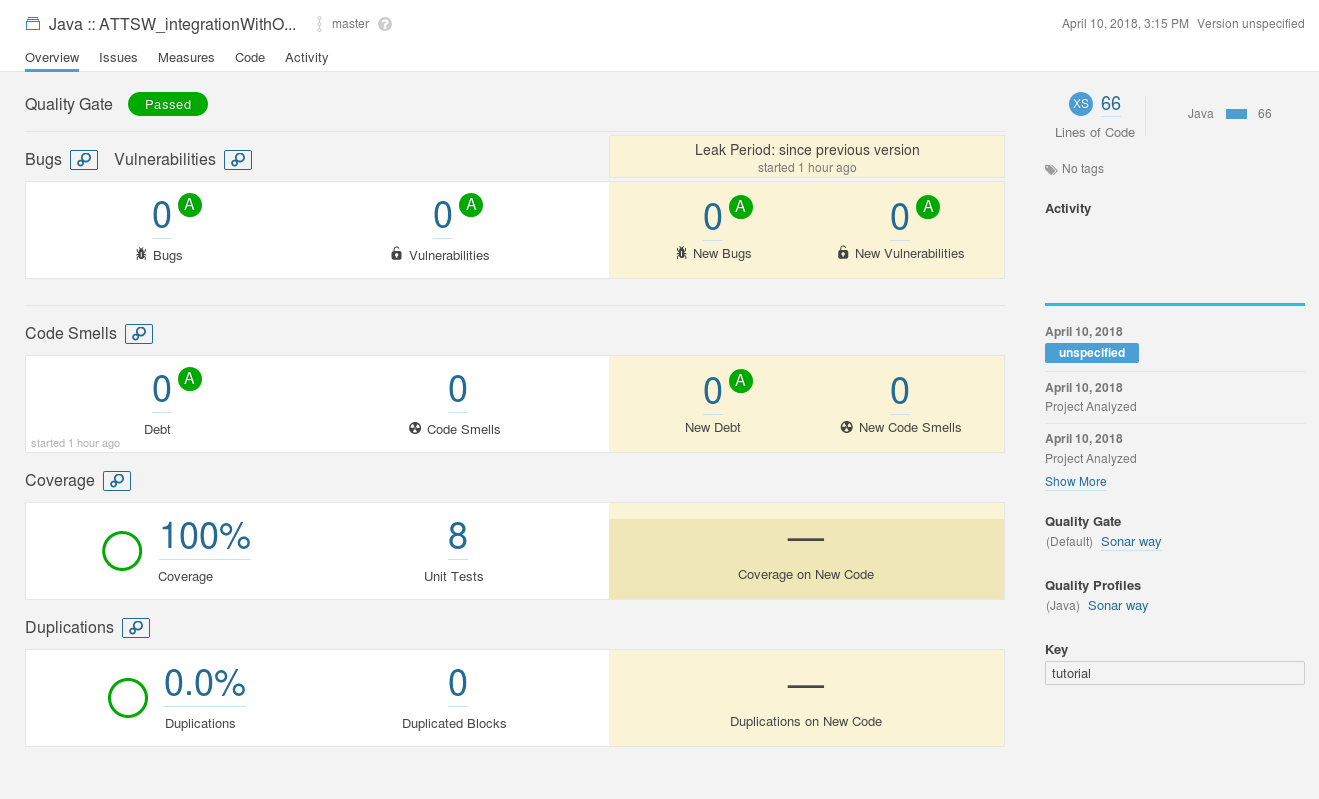
\includegraphics[width=0.8\linewidth]{4IntegrationWithOtherTool/tutorial/sonarqubeJacoco.png}
    \end{figure}
    \item Dal terminale possiamo eseguire il comando:
    \begin{verbatim}
        $ docker ps -a
    \end{verbatim}
    in output avremo tutti i contenitori attualmente attivi sulla nostra macchina, nel nostro caso avremo 2 contenitori corrispondenti alle immagini: sonarqube e postgress (database server usato da sonarqube). Una volta completata la nostra analisi del codice è possibile stoppare il contenitore e eliminarlo. Stoppiamo prima il contenitore del database e poi quello di sonarqube:
    \begin{verbatim}
        $ docker stop <nome_del_contenitore>
    \end{verbatim}
    una volta stoppati eliminiamoli usando il comando:
    \begin{verbatim}
        $ docker rm <nome_del_contenitore>
    \end{verbatim}
\end{enumerate}